\section{Proposed Research}
\label{sec:proposedresearch}

At the best of our knowledge there are not, out there, OpenMP data race
detectors that guarantee low runtime and memory overhead while maintaining
high precision and accuracy.
%
This motivate the need for better data race detection techniques and tools for
structured parallel programming paradigms.
%
As claimed in \S~\ref{sec:introduction}, we propose several different
contributions to obtain a better data race detection tool for OpenMP programs.
%
In the remainder of this section I will discuss and detail our proposed
contributions and how the combination of them helps to obtain a better OpenMP
data race detector.

\textbf{Sequential Blacklisting:} We exploit OpenMP's structured parallelism
to identify guaranteed sequential regions within OpenMP code.
%
Such analysis would be difficult to conduct in the context of unstructured
parallelism (e.g., PThreads).
%
Figure~\ref{fig:nested} shows an example of OpenMP parallel and nested
parallel regions.
%
As we can see, the parallel regions are alternated by the solely main thread
execution.
%
The code executed by the main thread is sequential and cannot race with any
other threads existing in a parallel region.
%
Therefore, the instructions executed by the main thread during its sequential
execution can be excluded from the runtime analysis reducing the overhead.

\begin{figure}
  \centering
  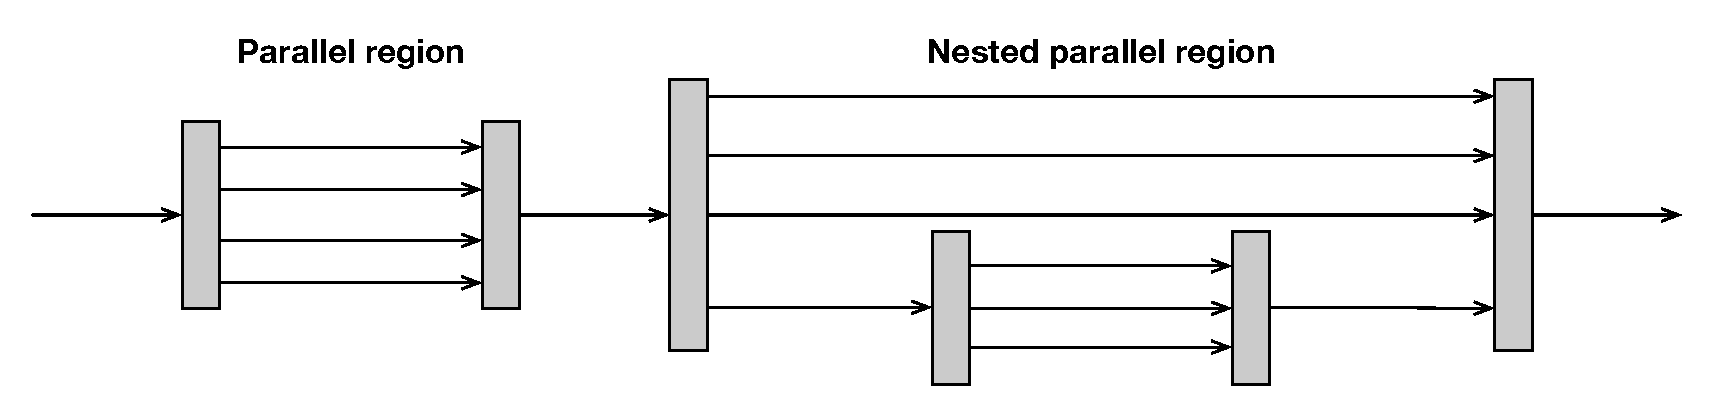
\includegraphics[width=0.95\textwidth]{figures/nested_parallelism}
  \caption{OpenMP nested parallelism}
  \label{fig:nested}
\end{figure}

\textbf{Data Dependency Analysis:} We identify and suppress race free parallel
loops from race checking.
%
Listing~\ref{code:example01} shows an example of two parallel for-loops.
%
The first one is easily and automatically parallelizable, the array will be
divided in different chunks and each of them will be assigned to different
threads.
%
However, the second parallel for-loops has a data dependency in the array
accesses, which will introduce a data race when the array's chunks are
assigned to different threads.
%
Indeed, it may happen that two threads will access the same locations
simultaneously without any synchronization mechanism.
%
The OpenMP compiler do not apply any check and will parallelize both loop in
the same way.
%
We introduce a data dependency analysis at compiling time that identify loops
with and without dependencies.
%
The firsts will be blacklisted and excluded by the runtime analysis since race
free, the seconds instead will be checked at runtime.

\begin{wrapfigure}{R}{0.37\textwidth}
  \vspace{-2ex}
  \begin{lstlisting}[language=C++, caption=OpenMP loops with and without loop-carried data dependency., label=code:example01]
  #pragma omp parallel for
  for(int i = 0; i < N; i++) {
    a[i] = a[i] + 1;
  }

  #pragma omp parallel for
  for(int i = 0; i < N; i++) {
    a[i] = a[i + 1];
  }
  \end{lstlisting}
\end{wrapfigure}

\textbf{\archer v1:} The two previous static analysis techniques and an
instrumented version of the OpenMP runtime make the first version of the
OpenMP data race detector \archer.
%
The static analyses will be implemented as a LLVM/Clang passes and integrated
in the compilation process.
%
We will annotate the OpenMP runtime to communicate the \tsan about the
happens-before relations between threads in presence of unknown
synchronization mechanisms.
%
For example, OpenMP barriers and OpenMP critical section are unknown to the
\tsan runtime, which would make it reports false positives.
%
This first version of \archer is the initial step towards low overhead data
race detector for large OpenMP applications, and it would also allow us to
evaluate the benefits of the static analyses in terms of both overheads
reduction, and precision and accuracy of the data race detection process.

\textbf{Clock-less runtime algorithm:} We design a 

I think we are totally avoiding vector/lamport clocks, instead using only the offset-span clocks and other info (barrier info). 
To me, this looks like THE DESIGN that one should follow.  The carry-over of
TSan is an overkill as the concurrency structure is much simpler for OMP.

\begin{itemize}
\item Barrier intervals
\item labeling to identify concurrent threads
\item sort of lock-set
\item Implemented by central but fast data structure
\item OMPT/OMPD
\end{itemize}

\textbf{\archer v2:} The second version of \archer will embed both static
analyses and the runtime analysis technique for data race detection of
structured parallelism.
%
We plan to integrate \archer in the LLVM/Clang compiler infrastructure and
guarantee the same ease to use that characterize most LLVM tools.
%
In fact, we will provide a new compilation flag (i.e. ``-archer'') that will
instrument the OpenMP program at compile time and will link it against the
\archer runtime library.
%
The program can then be executed as usual, while the \archer runtime library
will perform the data race detection providing at the end of the execution a
detailed report about the detected races.

\subsection{Evaluation}
\label{subsec:evaluation}

%%% Local Variables:
%%% mode: latex
%%% eval: (flyspell-mode 1)
%%% TeX-master: "root.tex"
%%% End:
